\documentclass[12pt]{article}
\usepackage{url, graphicx, epstopdf}

% page layout
\setlength{\topmargin}{-0.25in}
\setlength{\textheight}{9.5in}
\setlength{\headheight}{0in}
\setlength{\headsep}{0in}
\setlength{\parindent}{1.1\baselineskip}

% problem formatting
\newcommand{\problemname}{Problem}
\newcounter{problem}

% words
\newcommand{\foreign}[1]{\textsl{#1}}
\newcommand{\vs}{\foreign{vs}}

% math
\newcommand{\dd}{\mathrm{d}}
\newcommand{\e}{\mathrm{e}}

% primary units
\newcommand{\rad}{\mathrm{rad}}
\newcommand{\kg}{\mathrm{kg}}
\newcommand{\m}{\mathrm{m}}
\newcommand{\s}{\mathrm{s}}

% secondary units
\renewcommand{\deg}{\mathrm{deg}}
\newcommand{\km}{\mathrm{km}}
\newcommand{\cm}{\mathrm{cm}}
\newcommand{\mm}{\mathrm{mm}}
\newcommand{\ft}{\mathrm{ft}}
\newcommand{\mi}{\mathrm{mi}}
\newcommand{\AU}{\mathrm{AU}}
\newcommand{\ns}{\mathrm{ns}}
\newcommand{\h}{\mathrm{h}}
\newcommand{\yr}{\mathrm{yr}}
\newcommand{\N}{\mathrm{N}}
\newcommand{\J}{\mathrm{J}}
\newcommand{\eV}{\mathrm{eV}}
\newcommand{\W}{\mathrm{W}}
\newcommand{\Pa}{\mathrm{Pa}}

% derived units
\newcommand{\mps}{\m\,\s^{-1}}
\newcommand{\mph}{\mi\,\h^{-1}}
\newcommand{\mpss}{\m\,\s^{-2}}

% random stuff
\sloppy\sloppypar\raggedbottom\frenchspacing\thispagestyle{empty}

\begin{document}

\section*{NYU Physics I---Problem Set 10}

Due Thursday 2016 November 17 at the beginning of lecture.

\paragraph{\problemname~\theproblem:}\refstepcounter{problem}%
\textsl{(a)}~A figure skater spins in place on frictionless ice at
angular speed $\omega_i$ with her hands outstretched.  She has a total
moment of inertia $I_i$.  As the skater draws her hands into her body,
her moment of inertia decreases to $I_f=I_i/2$.  Does her kinetic
energy $K$ increase, decrease, or stay the same?  If it increases,
where does the energy come from?  If it decreases, where does the
energy go to?  \emph{Explain all your answers concisely but clearly:
What is conserved? That is, think in terms of conserved quantities.}

\textsl{(b)}~Now estimate the moments of inertia: $I_i$ of an ice
skater with her hands outstretched, and $I_f$ of an ice skater with
her hands drawn in.  Is the factor of 2 used in part \textsl{(a)}
reasonable?

\paragraph{\problemname~\theproblem:}\refstepcounter{problem}%
\textsl{(a)}~Immediately after being hit, at $t=0$, a cue ball of mass
$M$ and radius $R$ slides along the felt at speed $v_i$, not rotating
at all.  As time goes on, the ball slows down (because of friction)
and, at the same time, starts to spin.  Draw a free-body diagram for
the cue ball.  At what time $t_\mathrm{r}$ does the ball get to the
situation of ``rolling without slipping''?  Assume that there is a
coefficient $\mu$ of sliding friction. You will have to look up (or
compute) the moment of inertia $I$ for a uniform sphere.

\textsl{(b)}~Plot $v(t)$ and $R\,\omega(t)$ vs $t$ on a single plot.
\emph{Note that the two things I have asked you to plot have the same
dimensions.}  Clearly label $t_\mathrm{r}$ on your diagram.

\paragraph{\problemname~\theproblem:}\refstepcounter{problem}%
\textsl{(a)}~A hockey puck (a uniform disk of mass $m$, radius $r$,
and thickness $t$), slides without friction on ice with initial speed
$v_0$.  It strikes an identical puck tangentially, as shown in the
figure, and sticks to it.  The second puck is initially at rest and
also can slide without friction.  What is the final (linear) velocity
(speed $v$ and direction) of the stuck-together pucks?  What is the
moment of inertia $I_f$ and final angular speed of rotation $\omega$
of the system around its center of mass?  What fraction of the initial
kinetic energy (if any) is lost; \textit{ie,} what is $[K_i-K_f]/K_i$?
\\ \rule{0.25\textwidth}{0pt}
\resizebox{0.50\textwidth}{!}{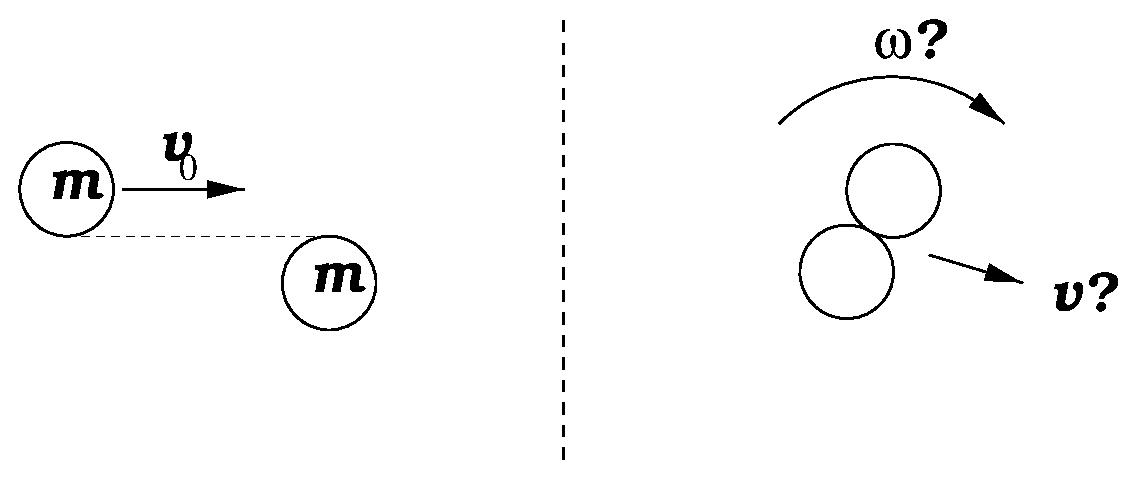
\includegraphics{tangpucks.eps}}
\\

\emph{Draw a clear diagram with a clearly labeled reference point used
to compute the angular momentum; recall that any angular momentum
calculation is with respect to your chosen origin.}

\textsl{(b)}~If the pucks had hit dead-on, the stuck-together pucks,
after the collision, would not be rotating.  Which of your answers
($v$, $\omega$, and $[K_i-K_f]/K_i$) will be different in this case?
If the fractional loss in kinetic energy is different, explain where
the difference in energy went.

\paragraph{Extra Problem (will not be graded for credit):}%
Between the initial hit of the cue ball by the cue---that is, when the
cue ball wasn't rotating at all---and the end of the cue ball
slide---that is, when the cue ball switches to rolling without
slipping---how much rotational kinetic energy ($I\,\omega^2 / 2$) was
created? How much linear kinetic energy ($m\,v^2 / 2$) was lost? How
much heat was generated? This extra problem refers to the pool problem
above.

\end{document}
